\question{\bfseries Intercept Meteor}

\subsection*{\sectionfont\upshape Background}

องค์การบริหารการบินและอวกาศแห่งโลกได้ตรวจพบอุกกาบาตขนาดใหญ่ที่กำลังพุ่งชนโลก 
จึงได้เตรียมแผนการรับมือโดยการส่งนักขุดเจาะฝีมือดีขึ้นไปวางระเบิดที่แกนของอุกกาบาตเพื่อระเบิดอุกกาบาตออกเป็นชิ้นเล็ก ๆ 
ก่อนจะตกลงสู่พื้นโลก จากการคาดการณ์ เศษอุกกาบาตส่วนใหญ่จะตกลงสู่ทะเล 
มีเพียงเกาะโคะเกาะเดียวเท่านั้นที่มีคนอาศัยอยู่และได้รับผลกระทบจากเศษอุกกาบาต

เพื่อปกป้องเกาะโคะที่มีอารยธรรมโบราณอันมีคุณค่า 
องค์การบริหารการบินและอวกาศแห่งโลกจึงได้ติดตั้งฐานยิงจรวดมิสไซล์ไว้ที่เกาะโคะเพื่อยิงเศษอุกกาบาตก่อนจะตกถึงพื้น
ข้อเสียของการใช้จรวดมิสไซล์คือ การยิงเศษอุกกาบาตแต่ละครั้งจะสร้างมลพิษสู่ชั้นบรรยากาศเป็นจำนวนมาก
องค์การบริหารการบินและอวกาศแห่งโลกจึงต้องการยิงเศษอุกกาบาตให้น้อยที่สุด
โดยจะยิงเฉพาะเศษอุกกาบาตที่มีจุดตกอยู่บนพื้นเกาะโคะเท่านั้น

ความพิเศษของเกาะโคะคือมีลักษณะเป็น convex polygon 
(เป็นรูปหลายเหลี่ยม และทุกคู่จุดใด ๆ บนเกาะสามารถเดินเป็นเส้นตรงถึงกันได้โดยไม่มีทะเลมาขวาง)

\subsection*{\sectionfont\upshape Problem Statement}

องค์การบริหารการบินและอวกาศแห่งโลกต้องการให้คุณเขียนโปรแกรมช่วยคำนวนว่าจากจุดตกของเศษอุกกาบาตแต่ละลูก 
มีลูกไหนตกบนพื้นเกาะโคะ, ตกตรงขอบเกาะโคะ และ ตกนอกเกาะโคะบ้าง

ให้พิจารณาเฉพาะ\uline{จุด}ตกเท่านั้น ไม่ต้องสนใจขนาดของเศษอุกกาบาต

\subsection*{\sectionfont\upshape Program Specification}

โปรแกรมที่คุณเขียนจะต้องอ่านข้อมูลจาก stardard input 
และเขียนคำตอบลง standard output โดยข้อมูลจะมีฟอร์แมตดังต่อไปนี้

\bigskip\noindent
{\sectionfont\bfseries Input Format}
\begin{itemize}
\item บรรทัดแรก เป็นจำนวนเต็มบวก $N$ แทนจำนวนมุมของ convex polygon $C$ ที่แสดงขอบเขตของเกาะโคะ
\item $N$ บรรทัดต่อมา แต่ละบรรทัดเป็นจำนวนเต็ม $x$ $y$ คั่นด้วยช่องว่าง 
    แทนพิกัดจุดมุมแต่ละจุดของ C เรียงตามเข็มนาฬิกา โดยเริ่มจากจุดที่มีค่า $x$ น้อยที่สุด 
    หากมีจุดที่มีค่า $x$ น้อยที่สุดมากกว่าหนึ่งจุดจะเริ่มต้นจากจุดที่มีค่า $y$ น้อยที่สุด 
    (รับประกันว่าไม่มีพิกัดใดซ้ำกันเลย และ ไม่มี 3 จุดมุมใดๆที่เรียงต่อเนื่องกันเป็นเส้นตรง)
\item บรรทัดต่อมา เป็นจำนวนเต็มบวก $K$ แทนจำนวนเศษอุกกาบาตที่ต้องการตรวจสอบ
\item $K$ บรรทัดต่อมา แต่ละบรรทัดเป็นจำนวนเต็ม $x$ $y$ คั่นด้วยช่องว่าง 
    แทนพิกัดของจุดตกของเศษอุกกาบาตที่ต้องการตรวจสอบแต่ละลูก
\end{itemize}

\medskip\noindent
{\sectionfont\bfseries Output Format}
สำหรับเศษอุกกาบาตที่ต้องการตรวจสอบแต่ละลูก ให้แสดงข้อความในหนึ่งบรรทัด โดยข้อความจะเป็น

\newpage
\begin{fullwidth}
    \begin{itemize}[itemsep=0pt]
        \item \lstinline|"Inside"| หากจุดตกอยู่ภายในเกาะโคะ หรือ
        \item \lstinline|"Outside"| หากจุดตกอยู่ภายนอกเกาะโคะ หรือ
        \item \lstinline|"On the boundary"| หากจุดตกอยู่บนเส้นรอบรูปของเกาะโคะพอดี 
        (อยู่บนขอบหรืออยู่ที่จุดมุมก็ได้)
    \end{itemize}
\end{fullwidth}

\subsection*{\sectionfont\upshape Data Example}
\begin{tabular}{p{0.45\linewidth}p{0.45\linewidth}}
\toprule
Example Input & Example Output \\
\midrule
\ttfamily\setstretch{0.8}
7 \newline
-5 1 \newline
0 6 \newline
6 10 \newline
10 11 \newline
10 9 \newline
5 4 \newline
0 2 \newline
6 \newline
0 5 \newline
-4 9 \newline
5 4 \newline
10 10 \newline
10 3 \newline
5 5 &
\ttfamily\setstretch{0.8}
Inside \newline
Outside \newline
On the boundary \newline
On the boundary \newline
Outside \newline
Inside \\
\bottomrule
\end{tabular}

\medskip\noindent
\textbf{อธิบายตัวอย่าง:} รูปล่างของเกาะโคะมีลักษณะดังที่ปรากฏทาง\ifpageodd{ขวา}{ซ้าย}มือ\;
นอกจากนั้นมี 6 คำถามดังต่อไปนี้
\marginnote{
    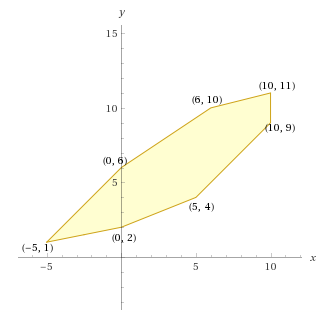
\includegraphics[width=0.96\linewidth]{figures/coding_national_interceptmeteor.png}
}
\begin{itemize}[itemsep=0pt]
\item คำถามแรก จุด (0, 5) อยู่ภายใน C ตอบว่า \lstinline|"Inside"|
\item คำถามที่สอง จุด (-4, 9) อยู่ภายนอก C ตอบว่า \lstinline|"Outside"|
\item คำถามที่สาม จุด (5, 4) เป็นจุดมุม ตอบว่า \lstinline|"On the boundary"|
\item คำถามที่สี่ จุด (10, 10) อยู่บนขอบ ตอบว่า \lstinline|"On the boundary"|
\item คำถามที่ห้า จุด (10, 3) อยู่ภายนอก C ตอบว่า \lstinline|"Outside"|
\item คำถามที่หก จุด (5, 5) อยู่ภายใน C ตอบว่า \lstinline|"Inside"|
\end{itemize}

\subsection*{\sectionfont\upshape Constraints}

โปรแกรมของคุณจะถูกทดสอบกับ test cases สองชุด (เรียกว่าชุดเล็ก และชุดใหญ่)
\begin{itemize}
\item test cases ชุดเล็กจะมีเงื่อนไขว่า จำนวนมุมของ convex polygon 
    ที่แสดงขอบเขตของเกาะโคะสอดคล้องกับเงื่อนไข $3 \leq N \leq 1,\!000$ 
    และจำนวนเศษอุกกาบาตที่ต้องการตรวจสอบสอดคล้องกับเงื่อนไข $1 \leq K \leq 1,\!000$
\item test cases ชุดใหญ่จะมีเงื่อนไขว่า จำนวนมุมของ convex polygon 
    ที่แสดงขอบเขตของเกาะโคะสอดคล้องกับเงื่อนไข $3 \leq N \leq 10^5$ 
    และจำนวนเศษอุกกาบาตที่ต้องการตรวจสอบสอดคล้องกับเงื่อนไข $1 \leq K \leq 10^5$
\item สำหรับทุก test cases จะมีเงื่อนไขว่า พิกัดจุดมุมของ convex polygon 
    ที่แสดงขอบเขตของเกาะโคะ และ พิกัดจุดตกของเศษอุกกาบาตสอดคล้องกับเงื่อนไข \\
    $-10^9 \leq x,y \leq 10^9$
\end{itemize}
